\ifx\wholebook\relax \else

\documentclass[b5paper]{ctexart}
\usepackage[nomarginpar
  %, margin=.5in
]{geometry}

\addtolength{\oddsidemargin}{-0.05in}
\addtolength{\evensidemargin}{-0.05in}
\addtolength{\textwidth}{0.1in}

\usepackage[cn]{../prelude}

\setcounter{page}{1}

\begin{document}

\title{零}

\author{刘新宇
\thanks{{\bfseries 刘新宇} \newline
  Email: liuxinyu99@hotmail.com \newline}
  }

\maketitle
\fi

\markboth{零}{数的旅程}

\ifx\wholebook\relax
\chapter{零}
\fi

\epigraph{因此“有”与“无”的真理,就是两者的统一。}{黑格尔《小逻辑》}

尽管数有超过5000年的历史,零却只有1200年的历史,是个“新生事物”。零诞生于印度,经由阿拉伯人引入欧洲。但它仅仅具有“占位符”的特殊身份,和1、2、3……比起来是个“二等公民”,甚至面临被“开除数籍”的风险。

\section{质疑与否定}
零一出生就代表“无”、“没有”。印度人给它起名叫sunya,意为“空位”。所以2025中的0表示\underdot{没有}百。“无\footnote{对应的英文是void,表示虚空。}”在西方的文化传统、宗教哲学上是负面否定的。它往往和黑暗、虚空、死亡等意象关联。而1代表\underdot{有}一个,2代表\underdot{有}两个……人们不说0,而说\underdot{没有},表示对\underdot{有}、\underdot{生存}、\underdot{实在}的否定。莎士比亚《王子复仇记》中的名句“To be or not to be, that is the question.”译为“生存还是死亡?”人们说3只羊跑了1只羊,还有两只羊;如果再跑了两只羊,人们说没有羊,而不说有0只羊。

\index{罗马算盘}
\begin{figure}[htbp]
 \centering
 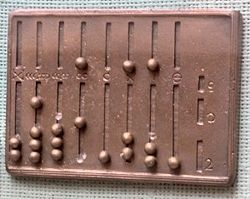
\includegraphics[scale=0.5]{img/Roman-abacus}
 \caption{现代复原的罗马算盘,在盘上开槽,槽中摆放石子,槽上标有罗马数字单位I, V, X, C, M。}
 \label{fig:roman-abacus}
 %https://www.newworldencyclopedia.org/entry/Abacus
\end{figure}

印度-阿拉伯计数系统传入欧洲后,尽管计算方便,人们还是把计算结果转换成罗马数字,而避免使用零\footnote{古代中国在进行算筹计算时(见第\ref{sec:counting-rods}节)用空位代表0。但计算完成后就把结果用乘法分组系统表示出来,如一百、两千一十五、一百有二。汉字“零”直到宋、元后才出现。}。教会宣布0是邪恶的符号,禁止在公开场合使用。僧侣学者们用算盘(如\cref{fig:roman-abacus},不是中国明代发明的珠算)计算。欧洲的算盘源自古巴比伦的泥板。就是在一块板上用小石子按照罗马数字演算,算好后抄下结果。但商人和银行家们看到了印度-阿拉伯数字的巨大好处,于是产生了十六世纪的“人机大战”,如\cref{fig:hindu-arabic-vs-abacus}。结果可想而知。自然是代表印度——阿拉伯计数的“机”胜了。这种“人机大战”在历史上一再上演:斯蒂芬森的火箭号列车\footnote{英国工程师乔治·斯提芬森和其子罗伯特·斯蒂芬森于1830年设计制造的蒸汽机车。}和马赛跑;深蓝挑战国际象棋大师卡斯帕罗夫;Alpha-Go挑战九段棋手李世石、柯洁;ChatGPT挑战大学生入学考试……每当有新事物出现,就有精彩的人机大战。

\begin{figure}[htbp]
 \centering
 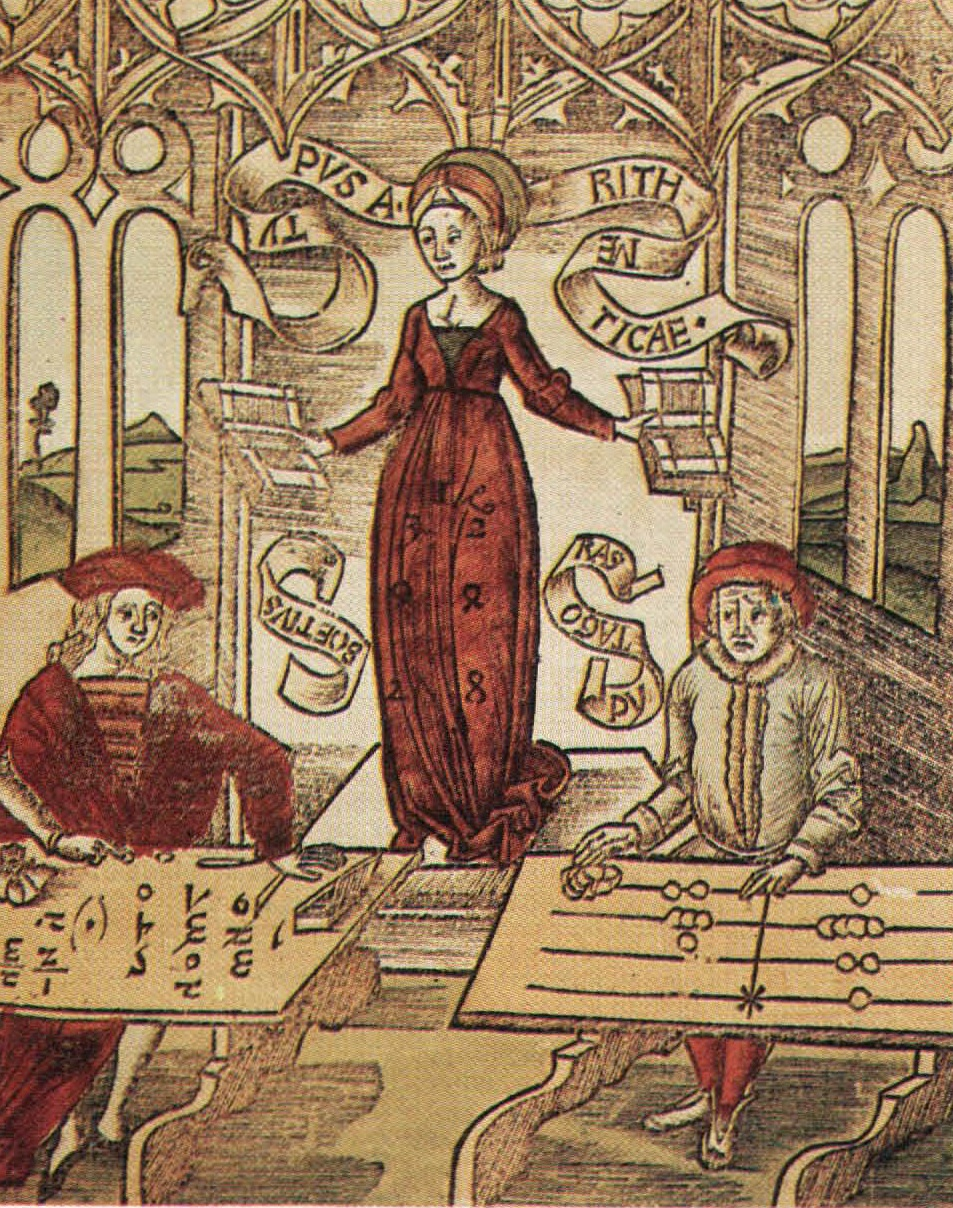
\includegraphics[scale=0.8]{img/Hindu-arabic-vs-abacus}
 \caption{1503年的版画。描绘了一个人用印度——阿拉伯数字计算,另一个人用罗马算盘计算的比赛。}
 \label{fig:hindu-arabic-vs-abacus}
 %https://www.newworldencyclopedia.org/entry/Abacus
\end{figure}

“机”的胜利让0具有了“二等公民”的身份——可以被使用了。可是为何0不能像1、2、3……那样成为“一等公民”呢?

\section{真正的数}

要想成为一等公民,0和1、2、3……比差了什么呢?是值,或者说大小。1这个符号代表的大小是1,比如1厘米的长度、1克的质量、1只羊……同样,2的值可以代表2厘米的长度、2克质量、2只羊……可是0呢?它没有值。“0是个占位符,不是一个数,因为它没有值\cite{Seife-2000}。”0极特殊,它表现得像一个破坏者,而非1、2、3……那样的“良民”。我们看看0是如何“破坏规矩”的:

\begin{enumerate}[(1)]
\item 阿基米德公理 \index{阿基米德公理}
\begin{align*}
1 + 1 &= 2   & 1 + 1 + 1 &= 3 & \dots \\
2 + 2 &= 4   & 2 + 2 + 2 &= 6 & \dots \\
3 + 3 &= 6   & 3 + 3 + 3 &= 9 & \dots \\
\dots &      & \dots     &    &
\end{align*}
一个数\footnote{本节的数都是自然数。}加上自己越来越大。阿基米德甚至指出这个规律是一个公理,今天叫做阿基米德公理:任意非零的$m < n$,则反复$m + m + \cdots$将会超过$n$。但 0 + 0 = 0没有变大,$0 + 0 + 0 + \cdots$不会超过任何数,包括1。

\item 积与面积

各个文明在丈量土地时都独立发展出了面积的概念,并将面积和乘法联系了起来。一块长方形的土地面积就是长与宽的积。$1 \times 5 = 5$代表宽1长5的矩形面积;$2 \times 5 = 10$代表宽2长5的矩形面积;$3 \times 5 = 15$代表宽3长5的矩形面积是……但是$0 \times 5$呢?矩形不见了,“坍缩”成了一个点\footnote{按欧几里得的定义,线段是没有宽度的,为什么矩形不是退化成了一条长5的线段?如果我们考虑长度的单位,例如厘米,则面积的单位是平方厘米。$0 \times 5 = 0$平方厘米,而线段只有长度,单位是5厘米。0平方厘米 $\neq$ 5厘米。},如\cref{fig:rectangle-vanish},矩形消失了。

\begin{figure}[htbp]
 \centering
 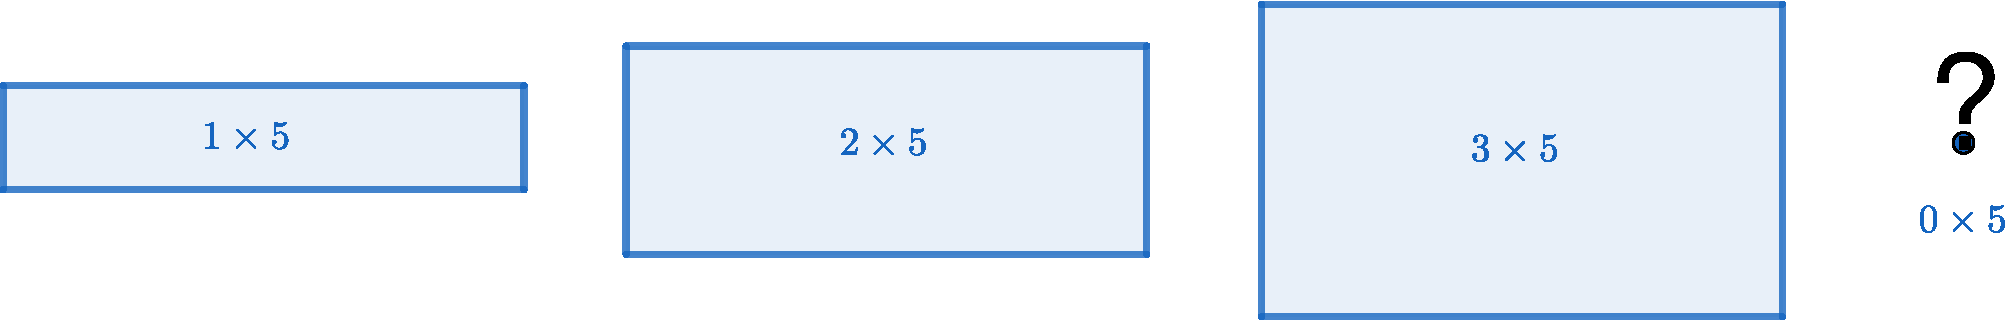
\includegraphics[scale=0.6]{img/rectangles}
 \caption{$0 \times 5$把矩形“压缩”成了一个没有大小的点。}
 \label{fig:rectangle-vanish}
\end{figure}

\label{sec:mul-as-zoom}
乘法还表示缩放。把一把尺子放大2倍,不仅尺子长度乘以2,尺子上的刻度间隔也乘以2;同样把尺子放大3倍,尺子的长度乘以3,刻度间隔也乘以3,如\cref{fig:ruler-vanish}。相反,把图中最大的尺子缩小3倍,即乘以$\frac{1}{3}$,则得到图中最小的尺子。但是如果缩放0倍(乘以0)整条尺子连同上面的刻度都“坍缩”成一点。尺子消失了。

\begin{figure}[htbp]
 \centering
 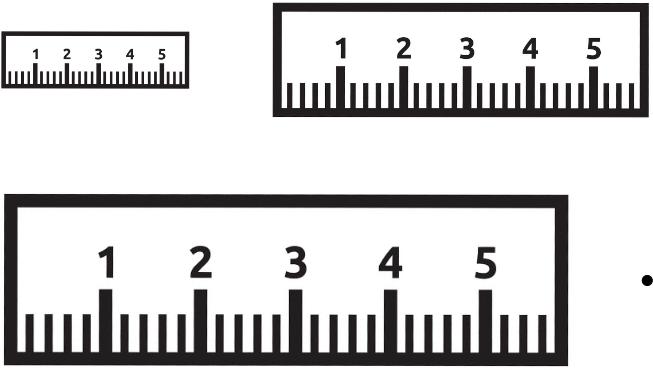
\includegraphics[scale=0.35]{img/zoom-rulers}
 \caption{缩放0倍把尺子连同刻度都“压缩”成了一个没有大小的点。}
 \label{fig:ruler-vanish}
\end{figure}

尺子代表了线段,乘以0破坏了矩形和线段。在古希腊发展几何学的时候还没有零的概念。古希腊的计数系统中也没有零。欧几里得定义“\textbf{点}是没有部分的”,“\textbf{线}只有长度而没有宽度”\footnote{欧几里得《几何原本》定义1、2。}。0对应几何学中的一个点么?

\item 乘除法的可逆性 \index{0!除数}

除法被定义为乘法的逆运算。既然$2 \times 3 = 6$则$6 \div 2 = 3$;既然$3 \times 4 = 12$则$12 \div 3 = 4$……据此$2 \times 0 = 0$则$0 \div 2 = 0$,并且$a \times 0 = 0$故$0 \div a = 0$。但是0可以作除数么?根据逆运算,除法$a \div b$相当于求$c$使得$bc = a$,则$a \div 0$相当于求一个数$x$使得$0x = a$。但$0x = 0$,若$a \ne 0$,则不存在任何数$x$满足这个要求,因为:$0x = 0 \ne a$;若$a = 0$,虽然$0 \times 0 = 0$,看似$0 \div 0 = 0$;但$1 \times 0 = 0$,这样$0 \div 0 = 1$看似也可以;同样$2 \times 0 = 0$,故似乎$0 \div 0 = 2$……既然任何$a \times 0 = 0$则$0 \div 0 = a$,即$0 \div 0$等于任何值。但这意味着$(0 \div 0) = 0 = 1 = 2 = 3 = \cdots$,代表“无”的0,等于代表“有”的1、2、3……无即是有,空即是色。逻辑学家罗素指出从一个假命题可以推出任何命题。如果$0 = 1$,我们可以推出$1 + 1 = 3$:

\begin{align*}
0 = 1 & \Rightarrow 1 = 2     & \text{两边} + 1 \\
      & \Rightarrow 1 + 1 = 3 & \text{把} 1 = 1 \text{加到两边}
\end{align*}

伊恩·斯图尔特给出了这样一个荒唐的例子\cite{Stewart-2019}:

一只猫有一只尾巴;

没有猫有八只尾巴。

把这两句话加起来:一只猫有九只尾巴。
\end{enumerate}

鉴于0的这些奇特的“破坏”性质,人们把0归为1、2、3……之外的异类,如\cref{fig:keyboard}所示,0被放到了1到9的后面。

\begin{figure}[htbp]
 \centering
 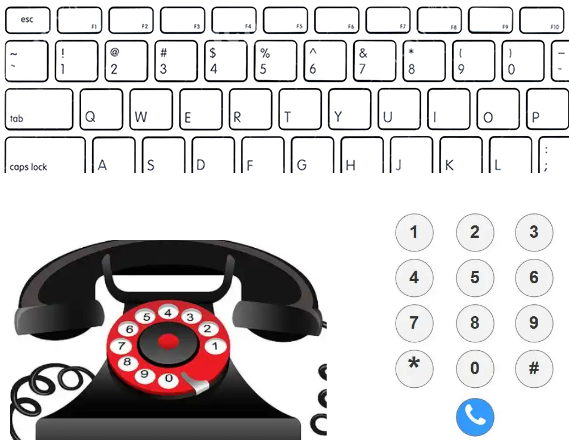
\includegraphics[scale=0.35]{img/keyboard}
 \caption{0在键盘上的位置}
 \label{fig:keyboard}
\end{figure}

\subsection{序数}
除了表示大小外,数还表示顺序。1、2、3……中,1在2的前面,3在2的右边。随着人们数数自然而然地感知到了顺序。迈克尔·阿廷在记下了他和女儿的对话\cite{MArtin-2011}:

“一、二、三、五、四……”

“不对,爸爸,应该是一、二、三、四、五”

“是的,但为什么我不能说一、二、三、五、四呢?”

“事情不是这样的。”

\begin{center}
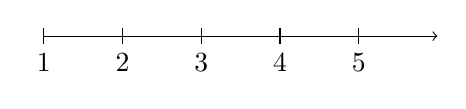
\begin{tikzpicture}
    \draw[->] (-2,0) -- (3,0); % node[right] {$x$};
    \foreach \x in {1,2,3,4,5}
    {
        \draw (\x-3,0.1) -- (\x-3,-0.1) node[below] {$\x$};
    }
    % \draw[fill=black] (-2,0) circle (0.05); % origin
\end{tikzpicture}
\end{center}

\index{数轴} \index{序数} \index{公元纪年}
把数字\underdot{按照顺序}排成一列叫做数轴。数的这种含义叫“序数”(ordinal)。在0引入西方前,制定历法的人不知道0的概念。于是规定:耶稣基督诞生后的年份为公元1年\footnote{耶稣生于12月25日,即西方的圣诞节。要到接下来的1月1日才算公元1年。},以后顺序为公元2年、公元3年……而之前的一年叫做公元前1年,再前一年叫公元前2年……注意这里没有零。这带来了一个有趣的问题,例如公元前202年5月,刘邦称帝建立西汉。到了公元9年正月王莽篡位西汉灭亡。那么西汉王朝有多长?如果用202 + 9 = 211年计算则多了1年。为了看出问题,我们只要考虑公元前1年12月25日出生的婴儿到了公元1年11月25日时几岁?当然不满1周岁,只有11个月大。那到了公元1年12月31日呢?有1岁了,但绝不可能是1 + 1 = 2岁。如果一个公元1年生的婴儿到了公元2年生日时几岁呢?2 - 1 = 1岁。一般公元$x$年到公元$y$年过了$y - x$年。那么1999年12月31日晚上11:59分50秒时,全世界都在倒数进入新千年。可严格说来公元2000年距公元1年过了2000 - 1 = 1999年。全世界提前庆祝了1年。为什么会有这个错误?因为跳过了公元0年(没有公元0年)。如果你没想明白,请考虑这个例子:午夜11点59分59秒后的1秒,标志着新的一天的开始。此时是\underdot{0}时0分0秒,新一天的第一秒是0时0分1秒。新的一天始于0时而不是1时。请仔细看看钟表盘。

\begin{figure}[htbp]
 \centering
 
\includegraphics[scale=0.35]{img/thermometer}
 \caption{温度计相当于一个垂直的数轴}
 \label{fig:thermometer}
\end{figure}

\index{温度}
我们看看温度计,如\cref{fig:thermometer}。一个大气压下冰水混合物的温度被定义为0$\degree$C;水沸腾的温度时100$\degree$C。之间均匀分成100份。1格代表1$\degree$C。这样温度计上的3对应的大小是3$\degree$C、4对应4$\degree$C……$x$对应$x \degree$C。零下5$\degree$C到10$\degree$C间差了15$\degree$C,避免了公元纪年出现的问题。如果把温度计横过来,我们就得到了一个正常的数轴。0处于1、2、3……的左侧。在这里0的含义不再是“无”,而是“起始”、“原点”。

\begin{center}
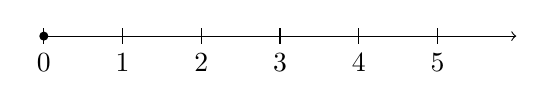
\begin{tikzpicture}
    \draw[->] (-3,0) -- (3,0); % node[right] {$x$};
    \foreach \x in {0,1,2,3,4,5}
    {
        \draw (\x-3,0.1) -- (\x-3,-0.1) node[below] {$\x$};
    }
    \draw[fill=black] (-3,0) circle (0.05); % origin
\end{tikzpicture}
\end{center}

\label{sec:zero-as-ordinal} \index{0!序数}
一个数$a$在$b$的左边,表明$a$在$b$之\underdot{前},即$a < b$,它们距离$b - a$。反之,$a$在$b$的右边,表明$a$在$b$之\underdot{后},即$a > b$,它们距离$a - b$\footnote{从节约一致的观点出发,我们可只用$a<b$定义“前”,用它的否定定义另一种情况。}。从运动的观点看$a + d$表示向前(右)移动$d$,$a - d$表示向后(左)移动$d$。如果$d = 0$,则$a + 0 = a - 0 = a$,表示固定$a$\underdot{不动}。在序数的意义下,0被赋予了合法的地位,不再是“二等公民”,而与1、2、3……一样是一个序数。

\index{数组}
在计算机系统中,有一种叫做数组(array)的数据结构。它使用一段连续的空间存储一组值,比如:

\begin{lstlisting}[language=C, frame=single]
int a[10];
\end{lstlisting}

声明一个数组$a$,它连续存储10个整数。在计算机内部,一个整数占16个二进制位,即用16个bit表示一个整数。对于正整数,最大可以表示到$2^{16}-1 = 65535$,即16个二进制位都是1。例如314写成二进制100111010(=256 + 32 + 16 + 8 + 2),即第9、6、5、4、2位是1,其它11位是0(见第\ref{sec:binary-numerals}节)。每8个二进制位称为一个字节(Byte),所以一个16位整数占用2个字节,记为:\lstinline|sizeof(int) = 2B = 16|。一个容纳10个整数的数组占用$2 \times 10 = 20$字节的存储空间。

计算机执行到\lstinline|int a[10]|时,就会在系统存储器\footnote{有两种情况:栈和堆。这个例子使用栈。}中找到一个位置,称为地址,让\lstinline|a|指向它。从这之后预留出连续20个字节来,供程序使用。接下来程序用这个地址索引数组的各个元素。比如从\lstinline|a|开始两个字节保存首个元素,\lstinline|a|后面第3、4字节保存次一个元素,如\cref{fig:array}把1、2……9、10存入了数组。

\begin{figure}[htbp]
 \centering
 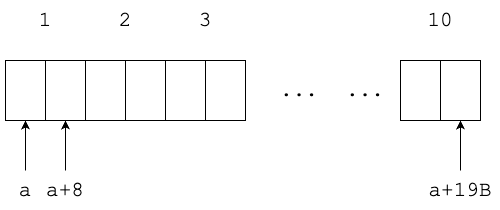
\includegraphics[scale=0.35]{img/array}
 \caption{数组}
 \label{fig:array}
\end{figure}

注意首个元素的地址从\lstinline|a|开始,它与地址\lstinline|a|的距离为0,记作\lstinline|a[0]|,次一个元素的地址从\lstinline|a + sizeof(int) = a + 16|开始,记作\lstinline|a[1]|,下一个地址从\lstinline|a + 2 * sizeof(int)|开始\footnote{计算机系统用“*”表示乘法},记作\lstinline|a[2]|……计算机从\lstinline|a + i * sizeof(int)|找到\lstinline|a[i]|,所以数组中的10个元素从0开始索引,依次是\lstinline|a[0], a[1], ..., a[9]|。很多人初学编程不知为何数组从0开始到$n-1$结束。其原因即在于此:数组的下标$i$表示了元素\lstinline|a[i]|到数组起始位置的\underdot{距离}。距离从0开始,0才是真正的起点。以下例子程序将1到10装入数组:

\begin{lstlisting}[language=C, frame=single]
int a[10];
for (int i = 0; i < 10; ++i) { a[i] = i + 1; }
\end{lstlisting}

有一个程序员自嘲的笑话。某程序员经过痛苦的熬夜加班,终得休息,决心全家吃顿饺子庆贺。他问孩子:“妈妈包了多少个饺子?”小孩子耳濡目染,指着盘中的饺子数道:“0、1、2、3……”妈妈无奈地感叹:“天生加班的程序员命。”

\index{植树问题}
类似的困扰也出现在小学数学中的“植树问题”中。一条100米长的路,每隔10米种一棵树,共需要几棵树?围绕400米长的操场跑道,每20米种一棵树,需要多少棵数?对于前者,我们只要把路想成数轴,意识到0是起点,从0数起:第0棵、第1棵、第2棵……第10棵。第$i$棵到起点的距离就是$10i$米。$100 \div 10 = 10$故第10棵树距起点100米。而0、1、2……10共11个数,故共种11棵数。对于后者,也从0开始数。400米是一圈,所以$400 \div 20 = 20$,第20棵树距离起点恰好是一圈400米,它和第0棵树位置重合,不需要种了,故0、1、2……19、$\cancel{20}$,共20棵树。

生活中我们一般从1开始数数1、2、3……,除了程序员和他可爱的孩子,似乎没有人从0开始数数。读者朋友们,你觉得什么情况下应该从1开始数,什么情况下应该从0开始数呢?(见\cref{qn:count-from})

\subsection{基数}
\index{基数}

从“无”到“起始”的变化是认识的转变,世界上各个文明对“无”有着不同的理解。基督教的创世纪神话描述世界开始之前是混沌与无,天地、光明、万物是世界的开始。佛教认为我们感知到的物质世界只是幻象,“无”才是世界的本质。古代中国在万物的变化中寻找规律,认为阴阳是推动变化的力量,从混沌的太极中演生大千世界。这些不同的认识和文化传统,导致了对于零的不同态度。随着东西文明的交融,人们对于无的认识也发生了变化。例如在西方哲学中,黑格尔系统地应用辩证法考虑绝对的有与绝对的无,并以纯粹的有无作为逻辑学的开始。今天的宇宙大爆炸理论认为我们的宇宙在诞生自138亿年前的一次大爆炸,根据相对论的观点,在此之前没有时间,没有空间。

\index{空集} \index{弗雷格}
既然代表“无”的0在序数上意味着起始,那么0在基数上是否可以“无中生有”呢?与序数对应的概念是基数(cardinal)。在前面的例子中,3的值可以代表3厘米的长度、3克的质量、3只羊……这些都是\underdot{具体}的大小。那么抽象的基数3,应该能代表任何包含3个事物的“复多”。用集合论的语言就是任何有3个元素的集合,如$\{\bigstar, \square, \bigcirc \}$或$\{a, b, c\}$。这正是逻辑学家弗雷格对抽象的数的定义。代表“无”的0是不包含任何元素的集合(即空集)的基数。布尔巴基学派在1939年用符号$\varnothing$代表空集。1是包含一个元素的集合的基数,一个元素的集合可以是$\{ \bigstar \}$、$\{ a \}$,甚至是$\{ \varnothing \}$。这是一个集合的集合,它包含的唯一元素是空集$\varnothing$。$\{ \varnothing \}$的基数是1。这样就用“无”构造出了“有”、从0到1。2是包含了两个元素的集合的基数。我们可以从1到2构造出$\{ \varnothing, \{ \varnothing \} \}$。它包含两个\underdot{不同}的元素(都是集合):空集$\varnothing$和$\{ \varnothing \}$。3是包含三个元素的集合的基数,可以从2到3构造出:$\{ \varnothing, \{ \varnothing \}, \{ \varnothing, \{ \varnothing \} \}\}$。以此类推。

\begin{tabular}{l|l}
  基数 & 集合 \\
  \hline
  0 & $\varnothing$ \\
  1 & $\{ \varnothing \}$ \\
  2 & $\{ \varnothing, \{ \varnothing \} \}$ \\
  3 & $\{ \varnothing, \{ \varnothing \}, \{ \varnothing, \{ \varnothing \} \}\}$ \\
  $\cdots$ & $\cdots$ \\
  $n$ & $\{ \varnothing, \{ \varnothing \}, \cdots \}$
\end{tabular}

这样就“无中生有”,以至万物;从0到1,从1到多。

\section{负数}
\index{负数}

0是打开魔盒的钥匙,它引发着人们的好奇心。一旦接受了0,自然就有这些问题:(1)1的前面是0,0的前面是谁?(2)1比2、3……小,0比1还小,还有比0更小的数么?(3)做减法$a -b$时,如果$b$比$a$还大会怎样?

\index{九章算术} \index{刘徽} \index{正负术}
到1500年左右,零已被人接受作为一个数,但负数的历史比零更短。16世纪和17世纪的大多数数学家并不承认它们是数\citepage[208]{MKlein-1972}。最早使用负数的是古代中国人。在汉代的《九章算术》中,已经有完整的“正负术”,如卷八中:“同名相除,异名相益……其异名相除,同名相益……”翻译成白话文的意思是:“(做减法时)正负相同值相减,正负相反值相加……(做加法时)正负不同值相减,正负相同值相加。”刘徽在注释中说:“今两算得失相反,要令正负以名之。正算赤,负算黑,否则以邪正为异。”翻译成白话文的意思是:“如果在计算中两个量所代表的意思相反,一个代表得到,一个代表失去,就需要用“正”、“负”来命名它们。用红色算筹表示正数,用黑色算筹表示负数(见第\ref{sec:counting-rods}节算筹部分)。如果手头没有不同颜色的算筹,就把一个正着放、一个斜着放加以区分。”\cite{Jiuzhang-2009}

可见中国古人在用算筹计算时,有两种不同颜色的算筹:红色代表正数,黑色代表负数。并形成了系统的计算规则。对正负数的实际意义也有解释,用正数表示卖出(对应收入),用负数表示买入(对应支出)。这既源于战国时代后日益繁荣的商业贸易,又源于传统思想文化中的阴阳概念。如\cref{fig:yinyang},红色的阳对应正,黑色的阴对应负。直到今天,我们仍然在医疗检测时说结果是阴性、阳性\footnote{阴性的英文为negative(负),阳性的英文为postive(正)。},在电化学中说电极是阴极、阳极。

\begin{figure}[htbp]
 \centering
 
\includegraphics[scale=0.1]{img/yinyang}
 \caption{阴阳}
 \label{fig:yinyang}
\end{figure}

\index{婆罗摩笈多}
古希腊文明将数的概念建立在几何之上。长度、面积、体积对应着几何图形的线段、形状、占据的空间。它们自然都是正的,没有形成负数的概念。伴随着十进制位值制系统和零的演进,印度数学在7世纪出现了负数。数学家婆罗摩笈多(公元589~670年)在他的著作中明确地区分正负数。他用财富和负债赋予正负数实际意义,使用特殊的符号标记负数,并给出了一系列的规则,如\cite{Rogers-2011}:

\begin{multicols}{2}
\begin{enumerate}[(1)]
\item 债务减零是债务。
\item 财富减零是财富。
\item 零减零为零。
\item 零减负债是财富。
\item 零减财富是负债。
\item 零乘以负债或财富是零。
\item 零乘以零为零。
\item 财富与财富的积或商是财富。
\item 负债与负债的积或商是财富。
\item 财富与负债的积或商是负债。
\item 负债与财富的积或商是负债。
\end{enumerate}
\end{multicols}

\begin{figure}[htbp]
 \centering
 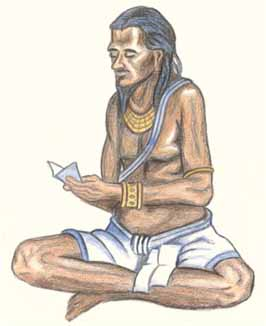
\includegraphics[scale=0.3]{img/Brahmagupta}
 \caption{婆罗摩笈多(安德里亚斯・施特里克绘)}
 \label{fig:yinyang}
\end{figure}

\index{丢番图} \index{卡尔达诺}
古希腊亚历山大时代的数学家丢番图(公元200~284年)开始独立于几何之外研究算术问题。他使用符号代表未知量,考虑了一次方程和二次方程的解。在他的著作《丢番图算术》中有一道题目:求方程$4 = 4x + 20$的解。面对引出的负数解,丢番图认为它是荒谬的。公元9世纪,阿拉伯数学家从印度的数学和天文学著作中接触到了负数,但他们同时又受到古希腊数学的影响,从而对负数产生了矛盾的态度。数学家花拉子密一方面接受负数的概念及其运算规则,并将其应用到解方程的移项与对消中,但另一方面,他使用几何论证方法的正确性,因此不得不排斥负数。花拉子密不能像我们今天一样用$ax + b = 0$概括所有一次方程,也不能能用$ax^2 + bx + c = 0$概括所有二次方程。为了避免负系数,他把方程划分为6类,如$ax = b$、$b - ax = 0$、$ax^2 + bx = c$、$bx + c = ax^2$、$ax^2 + c = bx$等。直到15世纪,欧洲学者才开始接触、研究负数。16世纪,意大利数学家卡尔达诺\footnote{也有人译作卡尔丹}(1501~1576年)在他的著作《大数》\footnote{拉丁文名为Ars Magna,出版于1545年。}中给出了一般三次、四次方程的公式解法。他同样遵循古希腊传统,使用几何证明正确性。把一次项解释为长度、二次项解释为面积、三次项解释为体积。不接受负数作为方程的系数。卡尔达诺不得不给出了60种不同类型的方程。

\subsection{序数}
\index{沃利斯} \index{数轴} \index{负序数}
17世纪,英国数学家沃利斯(1616~1703年)引入了数轴,并通过序数理解负数的意义。从序数上说,负数是0之前的部分,我们看下面两个例子。

\begin{example}
公元纪年。以耶稣基督诞生的一年为公元1年,此后为公元2年、3年……那么在耶稣诞生前呢?依然有时间,有历史事件发生。这些历史事件发生在公元前。耶稣诞生前的年份依次是公元前1年、公元前2年……公元前的年份蕴含着负数的意义(注意,这里缺少公元0年)。
\end{example}

\begin{example}
温度。进入冬天,气温逐渐下降,终于3度、2度、1度、0度,降到了冰点。但0度不是终结,尽管水凝固成冰,但随着温度继续下降,温度计上的红色煤油液面跨过了0度,降到了零下1度、零下2度……零下的温度比0度低,它们是负温度。
\end{example}

把温度计横过来,并向两边无限延伸,我们就得到了数轴:

\begin{center}
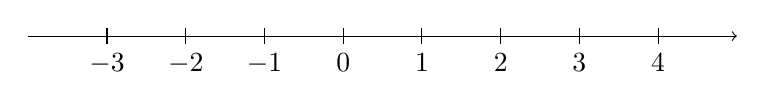
\begin{tikzpicture}
    \draw[->] (-4,0) -- (5,0);
    \foreach \x in {-3,-2,-1,0,1,2,3,4}
    {
        \draw (\x,0.1) -- (\x,-0.1) node[below] {$\x$};
    }
\end{tikzpicture}
\end{center}

负数作为序数在0和任何正数的左侧。0分开了正数、负数,位于中间。我们在第\ref{sec:zero-as-ordinal}介绍的规则依然成立:若$a < b$,$a$在$b$的左边,如果$b = 0$,$a$为负数,如果$a = 0$则$b$为正数。在序数意义下,小于“$<$”和大于“$>$”关系还可以用差的正负来表示。$a - b < 0$则$a < b$,$a$在$b$的左边\footnote{$a < b$,两边减$b$:$a - b < b - b = 0$}。$a - b > 0$则$a > b$,$a$在$b$的右边。若$d > 0$则$a + d$向前(右)移动$d$,$a - d$向后(左)移动$d$,若$a < d$,则移动到负数的区域。如果$d < 0$则移动的方向相反:$a + d$向后(左),$a - d$向前(右)。

\subsection{基数}
\index{负号}
尽管沃利斯用数轴给出了负数的意义,但他却奇怪地认为负数比无穷大,但不小于零。在《无穷大的算术》\footnote{拉丁文名为Arithmetica Infinitorum,1655年出版}中,沃利斯写到:由于比例$a/0$在$a$为正数时是无穷大\footnote{沃利斯是微积分的早期先驱之一,当时尚未形成严密的极限概念。若$a$、$b$都是正数,当观察到随着$b$减小到接近0时,$a/b$变得很大,于是随意地认为$a/0$是无穷大。},故当分母变为负数时,例如当$a/b$中的$b$是负数时,这个比必定大于无穷大\cite{MKlein-1972}。这都说明人们对于负数作为基数的意义感到困惑。总体来说,16世纪和17世纪,并没有很多数学家对于使用负数心安理得或者承认它是数,更谈不上承认它们可以作为方程的真实的根\cite{MKlein-1972}。笛卡尔的坐标系只有第一象限,帕斯卡则认为从0减去4纯粹是胡说。天文学家第谷·布拉赫使用了符号“-”来标识负数,但他认为负数只能私下使用。
%% https://web.ma.utexas.edu/users/mks/326K/Negnos.html

\index{绝对值}
负数引起的困惑是可以理解的。以温度为例,零下三十几度的南极洲显然比零下二十几度的东北地区更寒冷。从寒冷的程度看,如果基数表现大小,似乎南极洲温度的基数更大,但从数轴上的序数看$-30 < -20$。从年代上看,孔子(公元前551~公元前479年)生活的时代比孟子(公元前372~公元前289年)生活的时代更久远。如果基数表现大小,似乎孔子时代年份的基数更大,但从纪年的序数看$-479 < -372$。这些问题逐渐使我们认识到\underdot{绝对值}的概念。在数轴上,一个数$a$的绝对值是$a$到0的距离(长度),例如正数5的绝对值是$5 - 0 = 5$,即5本身;负数$-5$的绝对值是$0 - (-5) = 5$。在数轴上-5和5关于0对称,彼此称为对方的相反数。$a$的相反数是$-a$。而0到自己的距离是0 - 0 = 0。这样归纳下来,数轴上一个数$a$的绝对值记作$|a|$,有3种情况:

\[
|a| = \begin{cases}
  a & a > 0 \\
  0 & a = 0 \\
  -a & a < 0
\end{cases}
\]

\index{范·德·瓦尔登} \index{数偶}
用语言描述就是,正数和零的绝对值是它本身,负数的绝对值是它的相反数。二十世纪初,范·德·瓦尔登在《代数学》\footnote{原名《近世代数》。数学家范·德·瓦尔登当时从荷兰来到德国哥廷根求学,他根据埃米尔·阿廷和艾米·诺特的演讲和讨论班内容整理出了这本抽象代数讲义,影响了一代数学家。}一书中给出了一个“构造”负数的方法\citepage[8]{van-der-Waerden-2009}。用一对数偶$(a, b)$来表示整数如下:
\begin{itemize}
\item 用$(a + b, b)$表示自然数$a$。
\item 用$(b, b)$表示0。
\item 用$(b, a + b)$表示负数$-a$。
\end{itemize}

例如(3, 1)表示2, (5, 5)表示0,(100, 101)表示-1。我们可以把$(a, b)$想象成天平两边的质量,天平平衡时$(b, b)$两边质量相等,左右的的质量差为0;天平左侧质量更大的时候,左右质量差为正数;天平右侧质量更大的时候,左右质量差为负数。每个数都有许多表示,例如$(3, 1) = (9, 7) = (360, 358) = \cdots$都表示2;$(5, 5) = (100, 100) = (128, 128) = \cdots$都表示0;$(100, 101) = (1, 2) = (8, 9) = \cdots$都表示$-1$。但每个符号$(a, b)$定义一个,且只定义一个整数,即:

\begin{itemize}
\item 用$a > b$表示自然数$a - b$。
\item 用$a = b$表示0。
\item 用$a < b$表示负数$-(b - a)$。
\end{itemize}

接下来为数偶定义加法和乘法:

\begin{align}
(a, b) + (c, d) &= (a + c, b + d) \\
(a, b) \cdot (c, d) &= (ac + bd, ad + bc)
\label{eq:pair-add-mul}
\end{align}

例如加法$2 + (-1) = (5, 3) + (2, 3) = (7, 6) = 1$,乘法$-2 \times 3 = (1, 3) \cdot (5, 2) = (1 \times 5 + 3 \times 2, 1 \times 2 + 3 \times 5) = (11, 17) = -6$。\cref{qn:pair-arithmetic}要求读者验证加法、乘法的交换律、结合律、交换律(合称五大定律)对数偶都适用。

这个方法完全不使用零和负数,只用1、2、3……形式化地定义出了正数、零、负数,绕开了历史上引起争议的问题。不禁令人想起克罗内克的话:“上帝创造了自然数,其余都是人的工作。”

\section{数轴}
引入零和负数后,数轴上就标记出了向两侧无限延伸的整数。

\begin{center}
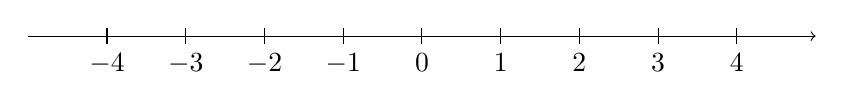
\begin{tikzpicture}
    \draw[->] (-5,0) -- (5,0);
    \foreach \x in {-4,-3,-2,-1,0,1,2,3,4}{
        \draw (\x,0.1) -- (\x,-0.1) node[below] {$\x$};
    }
\end{tikzpicture}
\end{center}

我们介绍一下标准符号的由来。0、1、2、3……叫做自然数,记作$\mathbb{N}$。是英文nature numbers的首字母。在没有认识到0以前,自然数不包括0,只有1、2、3……但随着0的引入,我们认识到0才是真正“自然”的起点、原点(见第\ref{sec:peano-axioms}节皮亚诺公理)。今天大多数定义(包括我国的部编义务教育数学教材)都把0算作自然数。通常用小写字母$n$表示某个自然数。引入负数后,负整数、零、正整数,即……$-3$、$-2$、$-1$、0、1、2、3……合称整数,记作$\mathbb{Z}$。它来自德语“数”Zahlen的首字母。正整数有时记作$\mathbb{Z}^+$,负整数记作$\mathbb{Z}^-$。整数的英文是integral number或integer,我们有时也用其首字母$i$表示某个整数。在枚举一些列的事物时,通常用$i$作下标,例如:$a_1, a_2, ..., a_i, ..., a_n$,其中$a_i$表示第$i$个。但这里的$i$不是integer,而是索引的英文index的首字母。$a_n$通常指最后一个,即第$n$个。数学家们非常重视符号的使用。好的符号形象、生动、易于理解,表达能力强,甚至具有意想不到的力量(如莱布尼茨的微积分符号)。韦达、笛卡尔开创了代数符号的传统,他们用$a, b, c$表示已知量,用$x, y, z$表示未知量。这些习惯影响至今。

\index{数轴!四则运算}
利用数轴,我们可以给出四则运算($+, -, \times, \div$)的直观解释(第3章会给出几何解释)。在\ref{sec:zero-as-ordinal}节,我们说加减$a \pm b$将数轴上的数$a$移动$b$个单位,共有五种移动情况:

\begin{center}
  \begin{tabular}{c|c|c|c}
          & $b > 0$ & $b < 0$ & $b = 0$ \\
  \hline
  $a + b$ & 向右     & 向左    & \multirow{2}{*}{不动} \\
  \cline{1-3}
  $a - b$ & 向左     & 向右
  \end{tabular}
\end{center}

我们看到$b < 0$时$a + b$相当于减法,而$a - b$相当于$a$加上$-b$。$b$和$-b$互为相反数,这样减法无非是加法的一种情况。我们可以用加法概括减法:

\begin{center}
\begin{tabular}{c|c|c|c}
        & $b > 0$ & $b < 0$ & $b = 0$ \\
\hline
$a + b$ & 向右     & 向左    & 不动
\end{tabular}
\end{center}

\begin{figure}[htbp]
 \centering
 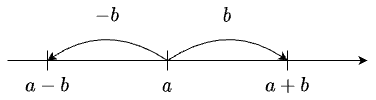
\includegraphics[scale=0.45]{img/translate}
\end{figure}

任给数轴上两个数$a, b$,它们的距离是:

\begin{center}
  \begin{tabular}{c|c|c|c}
      & $a < b$ & $a > b$ & $a = b$ \\
  \hline
  距离 & $b - a$ & $a - b$ & $0$
  \end{tabular}
\end{center}

\begin{figure}[htbp]
 \centering
 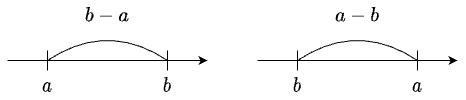
\includegraphics[scale=0.4]{img/distance}
\end{figure}

这恰是绝对值的概念,距离等于$|a - b|$。特殊情况下,若$b = 0$,一个数$a$到原点0的距离是$|a|$。

\begin{figure}[htbp]
 \centering
 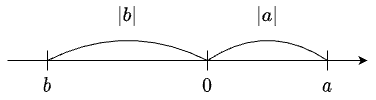
\includegraphics[scale=0.4]{img/abs}
\end{figure}

如果我们把“差”理解为“差距”,可正可负。在数轴上给定一个数$a$,它与另一个数$b$的差(距)就是$a - b$。若$a - b > 0$则$a > b$,$a$在$b$的右侧;若$a - b < 0$则$a < b$,$a$在$b$的左侧;若$a - b = 0$则$a = b$,$a$和$b$重合。特别地,$a$到原点0的差(距)$a - 0 = a$,就是它本身。

在数轴上,一个数$a$的相反数就是它关于原点0的对称点$-a$;0的相反数是它自己。

\begin{center}
\begin{tikzpicture}
    \draw[->] (-3,0) -- (3,0);
    \draw (-2,0.1) -- (-2,-0.1) node [below] {$-a$};
    \draw (2,0.1) -- (2,-0.1)   node [below] {$a$};
    \draw (0,0.1) -- (0,-0.1)   node [below] {$0$};
\end{tikzpicture}
\end{center}

0能“无中生有”:$0 \begin{cases} n \\ -n \end{cases}$,“分裂”成任何数$n$和它的相反数$-n$。反之,$n$和$-n$遇到一起“湮灭”为0,如同一对正负电荷。以上我们固定数轴,移动数轴上的数(点)。运动是相对的,我们也可以移动变换整条数轴:

\subsection{平移}
\index{数轴!平移}
把数轴上的\underdot{所有}数$+1$相当于把整条数轴怎样移动呢?向右?请看\cref{fig:plus-1-numline}:

\begin{figure}[htbp]
  \centering
  \begin{tikzpicture}{
      \draw[->] (-3,0) -- (4,0);
      \foreach \x in {-2,-1,0,1,2,3}{
          \draw (\x,0.1) -- (\x,-0.1) node[below] {$\x$};
      }
      \draw[fill=black] (0,0) circle (0.05); % origin

      \pgfmathsetmacro{\k}{-2}
      \draw[->] (-3,0+\k) -- (4,0+\k);
      \foreach \x in {-2,-1,0,1,2,3}{
          \pgfmathtruncatemacro{\y}{\x+1}
          \draw (\x,0.1+\k) -- (\x,-0.1+\k) node[below] {$\y$};
      }
      \draw[fill=black] (0-1,0+\k) circle (0.05); % origin
      \draw[->, decorate, decoration={snake, amplitude=.4mm, segment length=2mm, post length=1mm}]
        (0,0-0.8) -- (0,0+\k+0.3) node[above right] {$+1$};
  }
  \end{tikzpicture}
  \caption{将数轴上每个数$+1$}
  \label{fig:plus-1-numline}
\end{figure}

奇怪,竟然向左移动了1格。$\{\cdots -2, -1, 0, 1, 2 \cdots \}$各自加1后变成了$\{\cdots -1, 0, 1, 2, 3 \cdots \}$,的确向左移动了1个单位。那么$-1$一定是反向,也就是向右移动了,如\cref{fig:minus-1-numline}。

\begin{figure}[htbp]
  \centering
  \begin{tikzpicture}{
      \draw[->] (-3,0) -- (4,0);
      \foreach \x in {-2,-1,0,1,2,3}{
          \draw (\x,0.1) -- (\x,-0.1) node[below] {$\x$};
      }
      \draw[fill=black] (0,0) circle (0.05); % origin

      \pgfmathsetmacro{\k}{-2}
      \draw[->] (-3,0+\k) -- (4,0+\k);
      \foreach \x in {-2,-1,0,1,2,3}{
          \pgfmathtruncatemacro{\y}{\x-1}
          \draw (\x,0.1+\k) -- (\x,-0.1+\k) node[below] {$\y$};
      }
      \draw[fill=black] (0-1,0+\k) circle (0.05); % origin
      \draw[->, decorate, decoration={snake, amplitude=.4mm, segment length=2mm, post length=1mm}]
        (0,0-0.8) -- (0,0+\k+0.3) node[above right] {$-1$};
  }
  \end{tikzpicture}
  \caption{将数轴上每个数$-1$}
  \label{fig:minus-1-numline}
\end{figure}

一般地,$+a$将数轴移动$-a$,$-a$将数轴移动$a$。

\begin{center}
  \begin{tabular}{c|c|c|c}
                   & $a > 0$ & $a < 0$ & $a = 0$ \\
  \hline
  $\mathbb{Z} + a$ & 向左     & 向右    & \multirow{2}{*}{不动} \\
  \cline{1-3}
  $\mathbb{Z} - a$ & 向右     & 向左
  \end{tabular}
\end{center}

这是为什么呢?记原数轴为$A$,移动后的数轴为$A'$。$A$上的每个数$x \rightsquigarrow x + a$,变成了$x' = x + a$,$A$上的$-a \rightsquigarrow -a + a = 0$,变成了$A'$上的原点。所以$A'$上的原点\underdot{对应}着原数轴上的$-a$。若$a > 0$,自然新原点(对应$-a$)在老原点(对应0)的左边,如\cref{fig:translate-number-line}。

\begin{figure}[htpb]
  \centering
  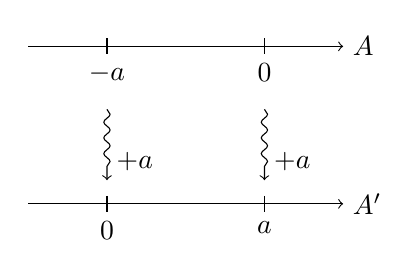
\begin{tikzpicture}{
      \draw[->] (-3,0) -- (1,0) node[right] {$A$};
      \draw (-2,0.1) -- (-2,-0.1) node[below] {$-a$};
      \draw (0, 0.1) -- (0, -0.1) node[below] {$0$};

      \pgfmathsetmacro{\k}{-2}
      \draw[->] (-3,0+\k) -- (1,0+\k) node[right] {$A'$};
      \draw (-2,0.1+\k) -- (-2,-0.1+\k) node[below] {$0$};
      \draw (0, 0.1+\k) -- (0, -0.1+\k) node[below] {$a$};

      \draw[->, decorate, decoration={snake, amplitude=.4mm, segment length=2mm, post length=1mm}]
          (-2,0-0.8) -- (-2,0+\k+0.3) node[above right] {$+a$};
      \draw[->, decorate, decoration={snake, amplitude=.4mm, segment length=2mm, post length=1mm}]
          (0,0-0.8) -- (0,0+\k+0.3) node[above right] {$+a$};
}
  \end{tikzpicture}
  \caption{数轴平移}
  \label{fig:translate-number-line}
\end{figure}

\subsection{相反数}
\index{相反数} \index{数轴!反向}
把数轴上的所有数取相反数(简称取反,英文negate)相当于把数轴反向(绕原点旋转$180\degree$)。

\begin{figure}[htpb]
  \centering
  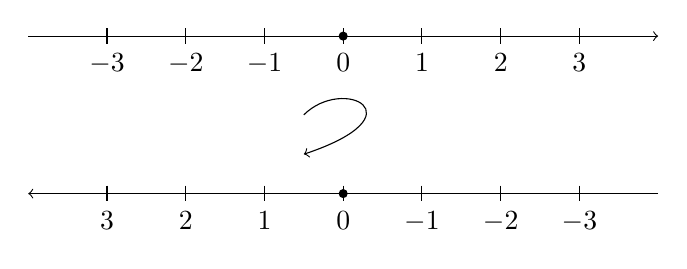
\begin{tikzpicture}{
      \draw[->] (-4,0) -- (4,0);
      \foreach \x in {-3,-2,-1,0,1,2,3}{
          \draw (\x,0.1) -- (\x,-0.1) node[below] {$\x$};
      }
      \draw[fill=black] (0,0) circle (0.05); % origin

      \pgfmathsetmacro{\k}{-2}
      \draw[->] (4,0+\k) -- (-4,0+\k);
      \foreach \x in {-3,-2,-1,0,1,2,3}{
          \pgfmathtruncatemacro{\y}{-\x}
          \draw (\x,0.1+\k) -- (\x,-0.1+\k) node[below] {$\y$};
      }
      \draw[fill=black] (0,0+\k) circle (0.05); % origin
      \draw[->] (-0.5, -1) .. controls (0, -0.5) and (1, -1.0) .. (-0.5, -1.5);
  }
  \end{tikzpicture}
  \caption{数轴反转}
  \label{fig:negate-number-line}
\end{figure}

取两次反自然会复原,即旋转$180\degree$再旋转$180\degree$等效于旋转$360\degree$,等效于不动。

\btab{ccccc}
  $\rightarrow$ & 反向 & $\leftarrow$ & 反向 & $\rightarrow$ \\
\hline
  $a$           & 相反数 & $-a$       & 相反数 & $-(-a) = a$
\etab

取相反数$a \rightsquigarrow -a$等效于乘以$-1$,即$-a = a (-1) = (-1) a$,两次取反复原就解释了“负负为正”:$-(-a) = (-1)(-a) = a$。

\subsection{缩放}
\index{数轴!缩放}
第\ref{sec:mul-as-zoom}节说乘除相当于缩放。$\times 2$把数轴放大2倍,$\times 3$把数轴放大3倍,$\div 2$把数轴缩小到$\frac{1}{2}$,$\div 3$缩小到$\frac{1}{3}$。除法是乘法的逆运算,所以$\div 2$也可以认为是$\times \frac{1}{2}$,即缩放到$\frac{1}{2}$倍,$\div 3$即缩放到$\frac{1}{3}$。这样乘除法就统一成乘法一种情况:

\begin{center}
  \begin{tabular}{c|c|c|c}
             & $a > 1$ & $0 < a < 1$ & $a = 1$ \\
  \hline
  $\times a$ & 放大     & 缩小    & 不变 \\
  \end{tabular}
\end{center}

引入负数后,如上节所说,$\times (-1)$相当于取相反数,数轴反向。$\times (-2)$相当于放大2倍后反转数轴,即$(-1) \times 2$,当然也等效于先反转数轴再放大2倍,即$2 \times (-1) = (-1) \times 2$。同样$\times (-3)$相当于放大3倍后反向,或反向后放大3倍。这样乘除法可以归纳如下:

\begin{center}
  \begin{tabular}{c|c|c|c|c|c|c}
             & $a > 1$ & $a = 1$ & $0 < a < 1$  & $-1 < a < 0$ & $a = -1$ & $a < -1$ \\
  \hline
  $\times a$ & 放大     & 不变    & 缩小          & 缩小 + 反向 & 反向 & 放大 + 反向
  \end{tabular}
\end{center}

有一种特殊情况:$\times 0$数轴“坍缩”成一点。上述“动作”可以组合:先平移$a$再平移$b$,当然这等效于先平移$b$再平移$a$,即$a + b = b + a$,这说明了加法的交换律。同样,先缩放$a$倍,再缩放$b$倍和先缩放$b$倍,再缩放$a$倍等效,即$ab = ba$,这说明了乘法交换率。我们把结合率的数轴意义作为\cref{qn:assiciative-numline}。

更复杂的组合,如先平移再缩放或反向,如$x \rightsquigarrow ax + b$,即先缩放$a$倍,再平移$-b$。\cref{qn:transform-numline}要求读者考虑如何先平移再缩放。

\section{单位元}
\index{单位元}
0和负数成了1、2、3……一样的一等公民。它们有序数(再数轴上合法、确定的位置),有基数(确定的值)。0和其它数比起来仍是如此特殊。它是起点,它是原点,它是产生万物的“无”,还有谁像它这样独特么?1站了出来要和0比一比。

\begin{align*}
  0     &             &  1 & \\
  1 + 0 & = 0 + 1 = 1  &  1 \times 0 &= 0 \times 1 = 0 \\
  2 + 0 &= 0 + 2 = 2  &  1 \times 2  &= 2 \times 1 = 2 \\
  3 + 0 &= 0 + 3 = 3  &  1 \times 3  &= 3 \times 1 = 3 \\
  \cdots &            & \cdots & \\
  a + 0 &= 0 + a = a  &  1 \times a  &= a \times 1 =  a
\end{align*}

0加上任何数都不变,而1乘以任何数(包括0)也都不变。我们看看0和1对数轴的作用:
\begin{enumerate}[(1)]
\item 加法把数轴左右平移,$+a$后数轴移动$-a$个单位($a > 0$向左,$a < 0$向右),0的作用是固定数轴不动。
\item 乘法把数轴放大缩小,$\times a$则缩放$a$倍($|a| > 1$放大,$0 < |a| < 1$缩小),1的作用是固定数轴不变。
\end{enumerate}

对于0,任何一个数$a$都能找到它的“加法双胞胎”兄弟,相反数$-a$,使得$a + (-a) = 0$。对于1,任何一个数$a$也能找到它的“乘法双胞胎”兄弟,倒数$\frac{1}{a}$,使得$a \times \frac{1}{a} = 1$,不过0没有“乘法双胞胎”兄弟。读者朋友们,你们觉得0和1谁更特殊呢?

像0和1这样“鹤立鸡群”的例子比比皆是。英语中有单词、短语、句子、段落……我们把一列英语字符叫做“字符串”,如``apple''、``hello''、``to be or not to be''、`` ''(空格)。我们可以把字符串连接在一起,如:``hello'' $\doubleplus$ `` '' = ``hello '',``hello '' $\doubleplus$ ``apple'' = ``hello apple''。不包含任何字符的串叫空串``'',把空串连接到任何字符上都不变:

\[
\text{``''} \doubleplus S = S \doubleplus \text{``''} = S
\]

如``'' $\doubleplus$ ``hello'' = ``hello'' $\doubleplus$ ``'' = ``hello''。再比如集合的并。把两个集合中包含的元素不重复地放在一起组成新的集合,如$\{a, b, c\} \cup \{1, 2, 3\} = \{a, b, c, 1, 2, 3\}$,$\{a, b, c\} \cup \{c, d, e\} = \{a, b, c, d, e\}$。空集与任何集合的并都不变:

\[
\varnothing \cup S = S \cup \varnothing = S
\]

如$\varnothing \cup \{a, b, c\} = \{a, b, c\} \cup \varnothing = \{a, b, c\}$。数学上我们把0叫做加法的单位元,1叫做乘法的单位元,空串叫做字符串连接的单位元,空集叫集合并的单位元。一般地在集合(可以有限也可以无限)$M$中,如果存在一个元素$e$,在某种二元运算$\odot$下使得:

\[
  e \odot a = a \odot e = a
\]
对$M$中的所有$a$都成立,我们把$e$叫做运算$\odot$在$M$中的单位元。例如0是加法在数的集合中的单位元,1是乘法在除去0之外的数的集合中的单位元,空串是连接操作在字符串集合中的单位元,空集是并在所有\underdot{集合的集合}中的单位元。单位元和集合中的其它元素一样是一等公民,但它是特殊的、唯一的(见\cref{qn:unique-e})。

\index{逆} \index{逆元}
对集合中的元素$a$,如果存在某个元素$b$使得$a \odot b = e$,则称$b$是$a$的逆。例如$a$在加法运算下的逆就是相反数$-a$,因为$a + (-a) = 0$。非0数$a$在乘法运算下的逆是$\frac{1}{a}$,因为$a \times \frac{1}{a} = 1$。并非所有元素都有逆,例如除了空串外,所有字符串都没有连接操作的逆;除了空集外,所有集合都没有并操作的逆。有了逆,我们就可以把加减乘除四则运算简化为“二则运算”,$a - b$只不过是$a$加上$b$的逆(相反数),$a \div b$只不过是$a$乘以$b$的逆(倒数)。

\section{皮亚诺公理}
\label{sec:peano-axioms}
1889年,意大利数学家皮亚诺为自然数建立起严格的公理化系统。它使用零作为起点,在加上“数数”这个动作,定义出了自然数。这组公理一共有五条,合称皮亚诺公理。

\index{皮亚诺公理}
\begin{enumerate}
\item 0是自然数。
\item (数数动作)每个自然数$n$都有它的下一个自然数$n'$,称为它的后继。
\end{enumerate}

似乎仅仅有这两条公理,已经能够定义出无穷无尽的自然数了,从0开始,下一个是1,下一个是2……接下来是某个$n$,下一个是$n+1$……以至无穷。但是好挑刺的数学家给出了一个反例:考虑只有两个元素$\{0, 1\}$组成的数字系统,定义1的后继为0,0的后继为1。这样也满足上面的两条公理,却不是我们想像中的自然数。为此我们还需要第三条皮亚诺公理来排除这种情况。

\begin{enumerate}
  \setcounter{enumi}{2}
  \item 0不是任何自然数的后继。
\end{enumerate}

仅仅有这三条公理就够了么?我们还可以给出一个反例:考虑有限元素$\{0, 1, 2\}$组成的数字系统,定义0的后继是1,1的后继是2,2的后继还是2。这样也能满足上述三条公理。为此我们还需要第四条皮亚诺公理。

\begin{enumerate}
  \setcounter{enumi}{3}
  \item 不同的自然数有不同的后继。如果两个自然数$m$和$n$的后继相同,则它们相等。即$m = n$当且仅当$m' = n'$;
\end{enumerate}

但是,仅仅用这四条公理仍然不够,因为存在这样的反例:考虑集合\{0, 0.5, 1, 1.5, 2, 2.5, ...\},定义0的后继是1、1的后继是2……,0.5的后继是1.5、1.5的后继是2.5……但0.5不是任何数的后继。为了排除这种“不可达”的数,还需要最后一条皮亚诺公理。

\begin{enumerate}
  \setcounter{enumi}{4}
  \item 如果自然数的某个子集$S$包含0,并且其中每个元素都有后继元素。那么$S$就是全体自然数$\mathbb{N}$。
\end{enumerate}

% 归纳公理(Axiom of induction)
\index{归纳公理} \index{数学归纳法}
为什么公理5可以排除掉上述反例呢?考虑$\{0, 0.5, 1, 1.5, 2, 2.5, ...\}$的一个子集$\{0, 1, 2, ...\}$。它包含0,并且每个元素都有后继元素,但是它不等于原集合。因为1.5、2.5……都不在这个子集中。所以它不满足第五条公理。公理五还有另外一个响亮的名字——归纳公理,它可以这样被等价地描述:

\begin{enumerate}
  \setcounter{enumi}{4}
  \item 任意关于自然数的命题,如果证明了它对自然数0是对的,又假定它对自然数$n$为真时,可以证明它对$n'$也真,那么命题对所有自然数都真。(这条公理保证了数学归纳法的正确性)
\end{enumerate}

例如,我们想证明能爬上任意层的大厦。用数学归纳法证明需要两个步骤:1、证明我们能进入大楼一层大厅。2、证明在任一层楼我们有能力“更上一层楼”。以上就是完整的五条皮亚诺公理,也称为皮亚诺算术系统。利用皮亚诺公理,我们可以定义出加法和乘法。加法定义包含两部分:任何自然数和0相加不变;$a$和$b$的后继相加,等于$a+b$的后继,即:\index{自然数的加法}

\be
\begin{laligned}
a + 0  &= a \\
a + b' &= (a + b)'
\end{laligned}
\label{eq:peano-add}
\ee

我们来验证一下2+3。2是0的二重后继$0''$,3是0的三重后继$0'''$,根据加法定义2+3为:

\[
0'' + 0''' = (0'' + 0'')' = (0'' + 0')'' = (0'' + 0)''' = (0'')''' = 0'''''
\]

结果的确是0的五重后继,也就是5。我们接下来定义自然数的乘法:\index{自然数的乘法}

\be
\begin{laligned}
a \cdot 0 &= 0 \\
a \cdot b' &= a \cdot b + a
\end{laligned}
\label{eq:peano-multiply}
\ee

乘法定义也包括两部分:任何数乘以0为0;$a$和$b$的后继相乘等于$a$乘以$b$再加上$a$。其中第二部分可以解释为:$a \cdot (b+1) = a \cdot b + a \cdot 1$。我们可以验证一下$2 \times 3$:

\begin{align*}
0'' \times 0''' & = 0'' \times 0'' + 0'' = 0'' \times 0' + 0'' + 0'' = 0'' \times 0 + 0'' + 0'' + 0'' \\
                & = 0 + 0'' + 0'' + 0'' = 0'' + 0'' + 0'' = (0'' + 0')' + 0'' = (0'' + 0)'' + 0'' \\
                & = (0'')'' + 0'' = 0'''' + 0'' \\
                & = (0'''' + 0')' = (0'''' + 0)'' = (0'''')'' = 0''''''
\end{align*}

结果的确是0的6重后继。\index{加法结合律}
与通常的观念不同,加法和乘法的交换律、结合律既不是公理也不是公设。它们都是定理,可以用皮亚诺公理和定义证明。以加法结合律为例。结合律是说$(a + b) + c= a + (b + c)$。我们先证明当$c=0$时它是对的。根据加法定义的第一条规则:

\[
(a + b) + 0 = a + b = a + (b + 0)
\]

然后是递推步骤,假设$(a + b) + c = a + (b + c)$成立,我们要推出$(a + b) + c' = a + (b + c')$。

\begin{align*}
(a + b) + c' &= (a + b + c)' && \text{加法定义的规则二,反向} \\
             &= (a + (b + c))' && \text{递推假设} \\
             &= a + (b + c)' && \text{加法定义的规则二} \\
             &= a + (b + c') && \text{加法定义的规则二,反向} & \mbox{\qed}
\end{align*}

这样就证明了加法的结合律。但加法交换律的证明却并不简单,本书附录\ref{app:add-commutativity}给出了完整的证明。

\begin{mdframed}
\index{皮亚诺}

\begin{center}
 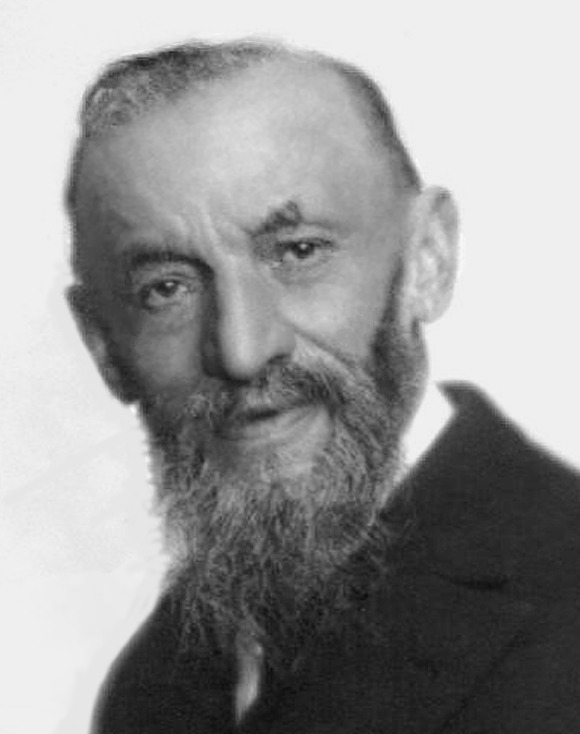
\includegraphics[scale=0.2]{img/Peano}
 \captionof{figure}{朱塞佩·皮亚诺(Giuseppe Peano)1858 - 1932。}
 \label{fig:Peano}
\end{center}

朱塞佩·皮亚诺1858年8月27日生于意大利库内奥(Cuneo)附近的斯宾尼塔(Spinetta)村。这是位于意大利北部都灵附近的农村。他出生的时候,正值意大利统一。1876年皮亚诺考入都灵大学学习,1880年毕业后就留校任教。皮亚诺最开始讲授微积分课程,1887年他和克罗西奥(Carola Crosio)结婚。1886年起,皮亚诺还同时担任都灵军事学院的教授。从19世纪80年代起,皮亚诺开始研究数理逻辑,并致力于数学基础的构建工作。他撰写了《数学公式汇编》这本巨著,力图把所有的数学成果都用形式化的方法汇集起来。这本书可以说为数学的严密化奠定了基础。1900年在第二届国际数学家大会上,罗素遇到了皮亚诺,他在自传(1951)中说\cite{M-Kline-2007}:

“这次大会是我的精神生活的一个转折点,因为在那里我遇到了皮亚诺。在此之前,我已经听说过他的名字,也知道他的一些工作。我突然明白了,他的符号提供了我多年来一直试图寻找的分析的工具,而且从他那里我获得了一直以来想要从事的工作的一种新的有效的技术。”

皮亚诺强烈地影响了罗素和怀特海合著的《数学原理》一书,对早期的计算理论起了重要的作用。皮亚诺最初用法语发表研究著作,但他对自然语言固有的歧义感到不满。为了解决这个问题,他于1900年左右发明了一套没有歧义的统一语言,称为“无屈折拉丁语”。这门语言后来被称为“国际语”(拉丁文Interlingua和世界语(Esperanto)是两种不同的人造语言)。皮亚诺努力推广他的新语言,但是事实并不如他所愿,几乎没有人愿意读他用国际语重写的《数学公式汇编》。相反倒是他早期的法语著作使数学家的观点发生了深刻的变化,尤其对法国的布尔巴基学派的纲领,产生了很大影响。1932年4月20日,皮亚诺因心脏病逝世于都灵。
\end{mdframed}

\begin{Exercise}[label={ex:zero}]
\Question{什么情况下应从1开始数数,什么情况下应从0开始数数?\label{qn:count-from}}
\Question{定义数偶的减法和除法}
\Question{验证数偶的加法乘法满足交换律、结合律、分配律\label{qn:pair-arithmetic}}
\Question{用乘法对加法的分配律证明$(-1) \times (-1) = 1$}
\Question{证明一个数的相反数是唯一的。}
\Question{说明加法、乘法结合律的数轴意义。\label{qn:assiciative-numline}}
\Question{考虑$x \rightsquigarrow 2x + 1$, 如果先平移再缩放,应先向哪个方向平移多少?再缩放几倍?一般地,$x \rightsquigarrow ax + b$应如何变换?\label{qn:transform-numline}}
\Question{证明单位元是唯一的。\label{qn:unique-e}}
\Question{定义0的后继为1,证明对于任何自然数都有$a \cdot 1 = a$}
\Question{证明乘法分配律。}
\Question{证明乘法结合律和交换律。}
\Question{如何利用皮亚诺公理验证3 + 147 = 150?}
\end{Exercise}

\begin{Answer}[ref={ex:zero}]
\Question{什么情况下应从1开始数数,什么情况下应从0开始数数?

考虑计数的情形是序数还是基数,是否包含到起点(原点)距离的含义,是否可能有负数的意义等因素。
}
\Question{定义数偶的减法和除法

  \begin{enumerate}[(a)]
  \item 减法相当于加上相反数,而数偶$(a, b)$的相反数是$(b, a)$。定义减法:$(a, b) - (c, d) = (a, b) + (d, c) = (a + d, b + c)$。
  \item 为了定义除法,注意到两个性质:(1)$(ka, kb)$相当于把$(a, b)$扩大$k$倍,$(\frac{1}{k}a, \frac{1}{k}b)$缩小到$\frac{1}{k}$。(2)$(-a, -b) = (b, a)$。利用它们得到:

    \[
    (a, b) / (c, d) = \begin{dcases}
        c > d: & (\dfrac{a}{c-d}, \dfrac{b}{c-d}) \\
        c < d: & (\dfrac{b}{d-c}, \dfrac{a}{d-c})
        \end{dcases}
    \]
    其中$c \ne d$。
  \end{enumerate}
}
\Question{验证数偶的加法乘法满足交换律、结合律、分配律
  \begin{enumerate}[(a)]
  \item 交换率:
    \begin{align*}
      (a, b) + (c, d) & = (a + c, b + d)  & \text{数偶加法定义} \\
                      & = (c + a, d + b)  & \text{自然数的加法交换律} \\
                      & = (c, d) + (a, b) & \text{反向用数偶加法定义}
    \end{align*}
    \begin{align*}
      (a, b) \cdot (c, d) & = (ac + bd, ad + bc) & \text{数偶乘法定义} \\
                          & = (ca + db, da + cb) & \text{自然数乘法交换律} \\
                          & = (c, d) \cdot (a, b) & \text{反向用数偶乘法定义}
    \end{align*}
  \item 结合律:略
  \item 分配律:我们只给出左侧分配律,略去右侧。
    \begin{align*}
         &(a, b) \cdot ((c, d) + (e, f)) & \\
        =& (a, b) \cdot (c + e, d + f) & \\
        =& (a(c + e) + b (d + f), a(d + f) + b(c + e)) & \\
        =& (ac + bd + ae + bf, ad + bc + af + be) & \\
        =& (ac + bd, ad + bc) + (ae + bf, af + be) & \text{反向用数偶加法定义} \\
        =& (a, b) \cdot (c, d) + (a, b) \cdot (e, f) & \text{反向用数偶乘法定义}
    \end{align*}
  \end{enumerate}
}
\Question{用乘法对加法的分配律证明$(-1) \cdot (-1) = 1$
  \begin{proof}
    \begin{align*}
      (-1) \times (-1) & = (-1) \times (-1) + 0 & \text{0加上任何数不变} \\
                      & = (-1) \times (-1) + (-1 + 1) & -1\text{和1互为相反数} \\
                      & = (-1) \times (-1) + (-1) \times 1 + 1 & \text{1乘以任何数不变} \\
                      & = (-1) \times (-1 + 1) + 1 & \text{反向用乘法分配律} \\
                      & = (-1) \times 0 + 1 = 0 + 1 = 1 & \qedhere
    \end{align*}
  \end{proof}
}

\Question{证明一个数的相反数是唯一的。
  \begin{proof}
    假设$b$是$a$的一个相反数,我们要证明$b = -a$:
    \begin{align*}
      0     & = b + a     & \text{相反数} \\
      0 - a & = b + a - a & \text{两边}-a \\
      -a & = b + (a - a)  = b + 0 = b & \qedhere
    \end{align*}
  \end{proof}
}

\Question{说明加法、乘法结合律的数轴意义。

加法:数轴先平移$a + b$再平移$c$等效于先平移$a$再平移$b+c$。乘法:数轴先缩放$ab$再缩放$c$等效于先缩放$a$再缩放$bc$。
}
\Question{考虑$x \rightsquigarrow 2x + 1$, 如果先平移再缩放,应先向哪个方向平移多少?再缩放几倍?一般地,$x \rightsquigarrow ax + b$应如何变换?

注意到$2x + 1 = 2(x + \frac{1}{2})$,所以先向\underdot{左}平移$\frac{1}{2}$再放大2倍。一般地,由于$ax + b = a(x + \frac{b}{a})$,故先平移$-\frac{b}{a}$(若$\frac{b}{a}>0$则向左,否则向右)再放大$a$倍。
}
\Question{证明单位元是唯一的。
\begin{proof}
假设存在另一单位元$e'$,使得对任意元素$a$满足$e' \odot a = a \odot e' = a$。我们要证明$e = e'$:
\begin{align*}
e &= e \odot e' & e'\text{是单位元} & \\
  &= e'         & e\text{是单位元}  &\qedhere
\end{align*}
\end{proof}
}

\Question{定义0的后继为1,证明对于任何自然数都有$a \cdot 1 = a$

\begin{proof}
利用\cref{app:add-commutativity}证明的结论:$0 + a = a$:

\begin{align*}
a' \cdot 1 & = a' \cdot 0' && \text{定义0的后继为1} \\
           & = a' \cdot 0 + a' && \text{乘法定义规则二} \\
           & = 0 + a' && \text{乘法定义规则一} \\
           & = a'
\end{align*}

\end{proof}
}
\Question{证明乘法分配律。

\begin{proof}
只证明左侧的分配律$c(a + b) = ca + cb$。对$b$使用数学归纳法,$b = 0$时:

\begin{align*}
c(a + 0) & = ca && \text{加法规则一} \\
         & = ca + 0 && \text{反向用加法规则一} \\
         & = ca + c0 && \text{反向用乘法规则一}
\end{align*}

递推假设$c(a + b) = ca + cb$,接下来证明$c(a + b') = ca + cb'$

\begin{align*}
c(a + b') & = c(a + b)' && \text{加法规则二} \\
          & = c(a + b) + c && \text{乘法规则二} \\
          & = ca + cb + c && \text{递推假设} \\
          & = ca + (cb + c) && \text{加法结合律} \\
          & = ca + cb' && \text{反向用乘法规则二}
\end{align*}
\end{proof}
}
\Question{证明乘法结合律和交换律。

我们只证明乘法结合律$(ab)c = a(bc)$,乘法交换律的证明则给出一个提纲。

\begin{proof}
对$c$使用数学归纳法,$c = 0$时:

\begin{align*}
(ab)0 & = 0 && \text{乘法规则一} \\
      & = a0 && \text{反向用乘法规则一} \\
      & = a(b0) && \text{反向用乘法规则一}
\end{align*}

递推假设$(ab)c = a(bc)$,接下来要证明$(ab)c' = a(bc')$

\begin{align*}
(ab)c' & = (ab)c + ab && \text{乘法规则二} \\
       & = a(bc) + ab && \text{递推假设} \\
       & = a(bc + b) && \text{上题证明的分配律} \\
       & = a(bc') && \text{反向用乘法规则二}
\end{align*}
\end{proof}

证明乘法交换律可以分为三步,都使用数学归纳法。首先证明$1a = a$,然后再证明右侧的分配律$(a + b)c = ac + bc$,最后再证明交换律。
}

\Question{如何利用皮亚诺公理验证3 + 147 = 150?

\vspace{3mm}
我们先看看经典的2 + 2 = 4是怎么证明的:

\begin{align*}
2 + 2 &=  0'' + 0'' && \text{2是0的两次后继} \\
      &=  (0'' + 0')' && \text{加法定义规则二} \\
      &=  ((0'' + 0)')' && \text{加法定义规则二} \\
      &=  ((0'')')' && \text{加法定义规则一} \\
      &=  0'''' = 4 && \text{0的4次后继}
\end{align*}

显然用这个方法证明3 + 147 = 150的话太冗长了,我们可以用先前证明的加法交换律证明147 + 3 = 150会容易一些。另一个方法是通过数学归纳法证明$3 + a = a'''$。
}
\end{Answer}

\ifx\wholebook\relax \else
\section{参考答案}
\shipoutAnswer

\section{加法交换律}
\subimport{inc/}{addcom-zh-cn}

\begin{thebibliography}{99}
\subimport{inc/}{bib-zh-cn}
\end{thebibliography}

\expandafter\enddocument
\fi
